\documentclass[12pt,a4paper]{scrartcl}\usepackage[]{graphicx}\usepackage[]{color}
%% maxwidth is the original width if it is less than linewidth
%% otherwise use linewidth (to make sure the graphics do not exceed the margin)
\makeatletter
\def\maxwidth{ %
  \ifdim\Gin@nat@width>\linewidth
    \linewidth
  \else
    \Gin@nat@width
  \fi
}
\makeatother

\definecolor{fgcolor}{rgb}{0.345, 0.345, 0.345}
\newcommand{\hlnum}[1]{\textcolor[rgb]{0.686,0.059,0.569}{#1}}%
\newcommand{\hlstr}[1]{\textcolor[rgb]{0.192,0.494,0.8}{#1}}%
\newcommand{\hlcom}[1]{\textcolor[rgb]{0.678,0.584,0.686}{\textit{#1}}}%
\newcommand{\hlopt}[1]{\textcolor[rgb]{0,0,0}{#1}}%
\newcommand{\hlstd}[1]{\textcolor[rgb]{0.345,0.345,0.345}{#1}}%
\newcommand{\hlkwa}[1]{\textcolor[rgb]{0.161,0.373,0.58}{\textbf{#1}}}%
\newcommand{\hlkwb}[1]{\textcolor[rgb]{0.69,0.353,0.396}{#1}}%
\newcommand{\hlkwc}[1]{\textcolor[rgb]{0.333,0.667,0.333}{#1}}%
\newcommand{\hlkwd}[1]{\textcolor[rgb]{0.737,0.353,0.396}{\textbf{#1}}}%
\let\hlipl\hlkwb

\usepackage{framed}
\makeatletter
\newenvironment{kframe}{%
 \def\at@end@of@kframe{}%
 \ifinner\ifhmode%
  \def\at@end@of@kframe{\end{minipage}}%
  \begin{minipage}{\columnwidth}%
 \fi\fi%
 \def\FrameCommand##1{\hskip\@totalleftmargin \hskip-\fboxsep
 \colorbox{shadecolor}{##1}\hskip-\fboxsep
     % There is no \\@totalrightmargin, so:
     \hskip-\linewidth \hskip-\@totalleftmargin \hskip\columnwidth}%
 \MakeFramed {\advance\hsize-\width
   \@totalleftmargin\z@ \linewidth\hsize
   \@setminipage}}%
 {\par\unskip\endMakeFramed%
 \at@end@of@kframe}
\makeatother

\definecolor{shadecolor}{rgb}{.97, .97, .97}
\definecolor{messagecolor}{rgb}{0, 0, 0}
\definecolor{warningcolor}{rgb}{1, 0, 1}
\definecolor{errorcolor}{rgb}{1, 0, 0}
\newenvironment{knitrout}{}{} % an empty environment to be redefined in TeX

\usepackage{alltt}
\usepackage[utf8]{inputenc}
\usepackage{amsmath}
\usepackage{graphicx}
\usepackage{tikz}
%\usepackage{silence}
\usepackage{mdframed}
%\WarningFilter{mdframed}{You got a bad break}
\usepackage[colorinlistoftodos]{todonotes}
\usepackage{listings}
\usepackage{color}
\colorlet{exampcol}{blue!10}
\usepackage{multicol}
\usepackage{booktabs}

\usepackage{exercise}

\usepackage[autostyle, english = american]{csquotes}
\MakeOuterQuote{"}

\usepackage{hyperref}
\hypersetup{
    colorlinks,
    citecolor=black,
    filecolor=black,
    linkcolor=blue,
    urlcolor=black
}

\title{Exercises for statistical inference and stuff}
\date{\today}
\author{Timoth\'ee Bonnet}
\IfFileExists{upquote.sty}{\usepackage{upquote}}{}
\begin{document}


\maketitle

\tableofcontents
\ListOfExerciseInToc
\ExerciseLevelInToc{subsubsection}


\section{Statistical inference and random numbers}

\subsection{Iris}
Some datasets are shipped with R (in R-base or in packages) and you can load them with the function data:

\begin{knitrout}
\definecolor{shadecolor}{rgb}{0.969, 0.969, 0.969}\color{fgcolor}\begin{kframe}
\begin{alltt}
  \hlkwd{data}\hlstd{(}\hlstr{"iris"}\hlstd{)}
\end{alltt}
\end{kframe}
\end{knitrout}
  
  The dataset looks like that:
  
\begin{knitrout}
\definecolor{shadecolor}{rgb}{0.969, 0.969, 0.969}\color{fgcolor}\begin{kframe}
\begin{alltt}
  \hlkwd{boxplot}\hlstd{(Sepal.Length} \hlopt{~} \hlstd{Species,}
      \hlkwc{data} \hlstd{= iris,}
      \hlkwc{drop} \hlstd{=} \hlnum{TRUE}\hlstd{,} \hlkwc{ylab}\hlstd{=}\hlstr{"Sepal length"}\hlstd{,} \hlkwc{xlab}\hlstd{=}\hlstr{"Species"}\hlstd{)}
\end{alltt}
\end{kframe}
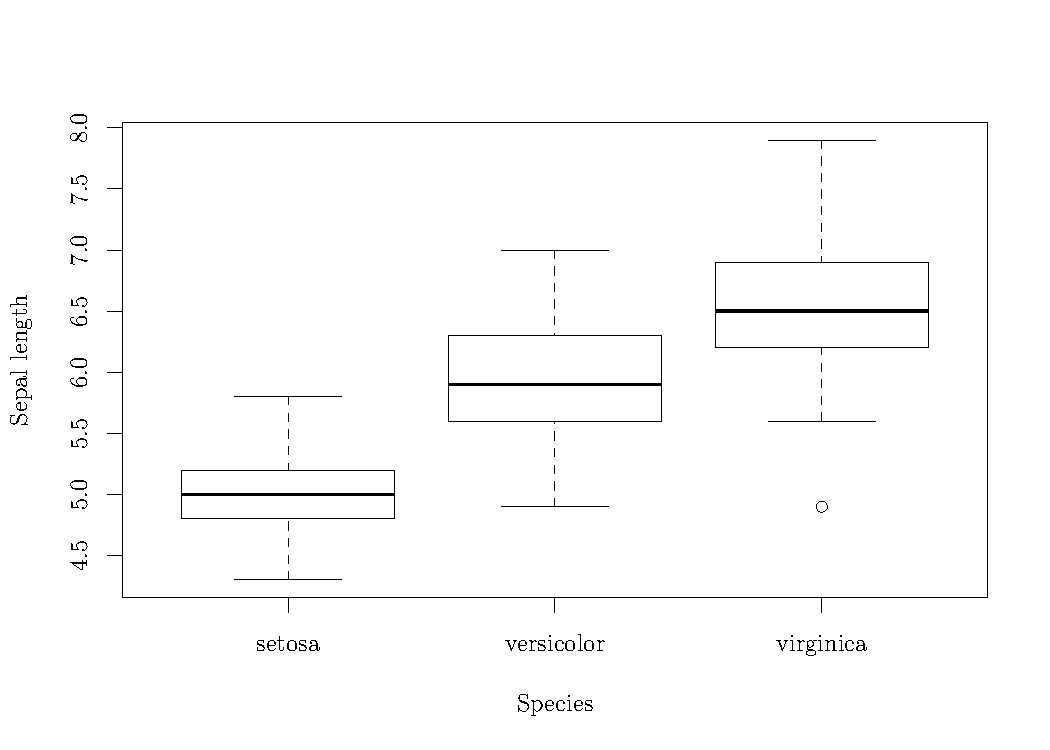
\includegraphics[width=0.7\textwidth,height=0.5\textwidth]{figure/boxplot-1} 

\end{knitrout}

\begin{Exercise}[difficulty=1]
\textbf{If you like ggplot, redo a boxplot of the iris data using that package.}
\end{Exercise}

\begin{Exercise}[difficulty=1]
\textbf{Do the species \emph{setosa} and \emph{versicolor} differ in their Sepal length? Use a t-test, an anova, and a linear model to answer. Compare the p-values between the three approaches.}
\end{Exercise}

\begin{Exercise}[difficulty=2]
\textbf{Now fit all species (\emph{setosa}, \emph{versicolor} and  \emph{virginica}) in a lm and an anova (you cannot fit a t-test with three levels) comparing Sepal length. Compare the model outputs, in particular the p-values. What is different, why?}
\end{Exercise}

\subsection{P-values and loops}

If we draw two sets of random numbers from the same normal distribution, we do not expect them to be associated. In the case below, the p-value for the slope of y on x is 0.802, non-significant.
\begin{knitrout}
\definecolor{shadecolor}{rgb}{0.969, 0.969, 0.969}\color{fgcolor}\begin{kframe}
\begin{alltt}
\hlkwd{set.seed}\hlstd{(}\hlnum{1234}\hlstd{)}
\hlstd{x} \hlkwb{<-} \hlkwd{rnorm}\hlstd{(}\hlnum{100}\hlstd{)}
\hlstd{y} \hlkwb{<-} \hlkwd{rnorm}\hlstd{(}\hlnum{100}\hlstd{)}
\hlkwd{summary}\hlstd{(}\hlkwd{lm}\hlstd{(y}\hlopt{~}\hlstd{x))}
\end{alltt}
\begin{verbatim}
## 
## Call:
## lm(formula = y ~ x)
## 
## Residuals:
##      Min       1Q   Median       3Q      Max 
## -2.88626 -0.61401  0.00236  0.58645  2.98774 
## 
## Coefficients:
##             Estimate Std. Error t value Pr(>|t|)
## (Intercept)  0.03715    0.10498   0.354    0.724
## x           -0.02608    0.10378  -0.251    0.802
## 
## Residual standard error: 1.037 on 98 degrees of freedom
## Multiple R-squared:  0.0006443,	Adjusted R-squared:  -0.009553 
## F-statistic: 0.06318 on 1 and 98 DF,  p-value: 0.8021
\end{verbatim}
\end{kframe}
\end{knitrout}

\begin{Exercise}[difficulty=2]
Are we every going to find a significant p-value with two sets of random numbers? Write a while loop to find out. How many iterations until you find a p-value below 0.05?
\end{Exercise}


\begin{Exercise}[difficulty=3]
How often do you observe a significant test with randomly drawn numbers? Use a for-loop to record the distribution of p-values. Does this distribution depend on the sample size of x and y? What does increasing sample size do to the significant tests?
\end{Exercise}

\section{R-studio tricks}

\subsection{Column selection}

\begin{Exercise}[difficulty=1]
Use the shortcut  \texttt{Alt+click} to change the code below so that you plot the five linear models defined at the beginning:
\begin{knitrout}
\definecolor{shadecolor}{rgb}{0.969, 0.969, 0.969}\color{fgcolor}\begin{kframe}
\begin{alltt}
\hlstd{lmadd}  \hlkwb{<-} \hlkwd{lm}\hlstd{(y} \hlopt{~} \hlstd{x1} \hlopt{+} \hlstd{x2)}
\hlstd{lmnull} \hlkwb{<-} \hlkwd{lm}\hlstd{(y} \hlopt{~} \hlnum{1}\hlstd{)}
\hlstd{lmff}   \hlkwb{<-} \hlkwd{lm}\hlstd{(y} \hlopt{~} \hlstd{x1}\hlopt{*}\hlstd{x2)}
\hlstd{lmx2}   \hlkwb{<-} \hlkwd{lm}\hlstd{(y} \hlopt{~} \hlstd{x2)}
\hlstd{lmx1}   \hlkwb{<-} \hlkwd{lm}\hlstd{(y} \hlopt{~} \hlstd{x1)}


\hlkwd{plot}\hlstd{(lm1)}
\hlkwd{plot}\hlstd{(lm2)}
\hlstd{...}
\end{alltt}
\end{kframe}
\end{knitrout}
\end{Exercise}
 
 \begin{Exercise}[difficulty=2]
 What if my code was not well aligned? 
Use \texttt{Ctrl + Alt + clicks} to create multiple cursors, then \texttt{Shift + Home} and \texttt{Ctrl + C}
\begin{knitrout}
\definecolor{shadecolor}{rgb}{0.969, 0.969, 0.969}\color{fgcolor}\begin{kframe}
\begin{alltt}
\hlstd{lmadd} \hlkwb{<-} \hlkwd{lm}\hlstd{(y} \hlopt{~} \hlstd{x1} \hlopt{+} \hlstd{x2)}
\hlstd{lmnull} \hlkwb{<-} \hlkwd{lm}\hlstd{(y} \hlopt{~} \hlnum{1}\hlstd{)}
\hlstd{lmff} \hlkwb{<-} \hlkwd{lm}\hlstd{(y} \hlopt{~} \hlstd{x1}\hlopt{*}\hlstd{x2)}
\hlstd{lmx2}\hlkwb{<-} \hlkwd{lm}\hlstd{(y} \hlopt{~} \hlstd{x2)}
\hlstd{lmx1}  \hlkwb{<-} \hlkwd{lm}\hlstd{(y} \hlopt{~} \hlstd{x1)}


\hlkwd{plot}\hlstd{(lm1)}
\hlkwd{plot}\hlstd{(lm2)}
\end{alltt}
\end{kframe}
\end{knitrout}
 \end{Exercise}

\subsection{Short-cuts}

R-Studio short-cuts are listed in Tools - Keyboard Shortcuts Help, also accessible using the shortcut \texttt{Alt + Shift + K}.

\begin{Exercise}[difficulty=1]
Read them, find one that would be helpful to you, and memorize it
\end{Exercise}

\section{Linear models}

\subsection{Diagnostics and assumptions}
\begin{Exercise}[difficulty=2]
\begin{enumerate}
    \item Load Cdata.csv
    \item fit a linear model of y as a function of x2 and x3. Something is weird, what is going on? How to interpret and what to do?
    \item fit a linear model of y as a function of x1 and x2. Something else is weird, what is going on? How to interpret and what to do?
  \end{enumerate}
\end{Exercise}

\begin{Exercise}[difficulty=2]
Load the dataset Anscombe.csv. It contains four sets of distributions for a x and a y variable. Create a subset of the data for each distribution, and fit a linear regression of y on x for each subset. 
\textbf{Compare the summaries. Use the function plot() to diagnose the models, and to visualize the data. Which models do you trust? For what?\\ Try and confirm your confidence in various models by ploting model predictions with confidence intervals and actual observations together.} 

\end{Exercise}


\subsection{Prediction}
  \begin{Exercise}[difficulty=2]
  What explains variation in parasitic load?
  You collected ecto-parasites on some furry large mammals at three locations. Parasites break easily when we collect them and are impossible to count, so we decide to measure parasitic load as their mass. \textbf{Why do some mammals have larger parasitic load?} 
    \begin{itemize}
      \item Load the \texttt{Para.csv} data (don't forget: str(), summary(), plot()\dots)
      \item Model \verb+Parasite_Mass+ using \texttt{lm()}
      \item Find what variables predict \verb+Parasite_Mass+
      \item How good are your models? Assumptions? Prediction?
      \item What biological interpretation can you imagine?
      \end{itemize}
    \end{Exercise}

\begin{Exercise}[difficulty=3]
Write your own code to obtain a prediction from a lm (that is, a simpler version of the predict function). Use any dataset to test it.
\end{Exercise}

\section{While-loop}

\subsection{What you need to know}
\begin{knitrout}
\definecolor{shadecolor}{rgb}{0.969, 0.969, 0.969}\color{fgcolor}\begin{kframe}
\begin{alltt}
    \hlkwd{while}(condition TRUE)
    \{
      something
    \}
\end{alltt}
\end{kframe}
\end{knitrout}
  
For instance:
\begin{knitrout}
\definecolor{shadecolor}{rgb}{0.969, 0.969, 0.969}\color{fgcolor}\begin{kframe}
\begin{alltt}
\hlstd{x} \hlkwb{<-} \hlnum{0}
\hlkwa{while}\hlstd{(x}\hlopt{<}\hlnum{10}\hlstd{)}
    \hlstd{\{}
      \hlstd{x} \hlkwb{<-} \hlstd{x}\hlopt{+}\hlnum{1}
      \hlkwd{print}\hlstd{(x)}
    \hlstd{\}}
\end{alltt}
\begin{verbatim}
## [1] 1
## [1] 2
## [1] 3
## [1] 4
## [1] 5
## [1] 6
## [1] 7
## [1] 8
## [1] 9
## [1] 10
\end{verbatim}
\end{kframe}
\end{knitrout}
  
  
\subsection{Practice}

The function sample() takes 5 number between 1 and 6 (like 5 dice!):
\begin{knitrout}
\definecolor{shadecolor}{rgb}{0.969, 0.969, 0.969}\color{fgcolor}\begin{kframe}
\begin{alltt}
\hlstd{x} \hlkwb{<-} \hlkwd{sample}\hlstd{(}\hlkwc{x} \hlstd{=} \hlnum{1}\hlopt{:}\hlnum{6}\hlstd{,} \hlkwc{size} \hlstd{=} \hlnum{5}\hlstd{,} \hlkwc{replace} \hlstd{=} \hlnum{TRUE}\hlstd{)}
\end{alltt}
\end{kframe}
\end{knitrout}

Are all die equal?
\begin{knitrout}
\definecolor{shadecolor}{rgb}{0.969, 0.969, 0.969}\color{fgcolor}\begin{kframe}
\begin{alltt}
\hlkwd{all}\hlstd{(x} \hlopt{==} \hlstd{x[}\hlnum{1}\hlstd{])}
\end{alltt}
\begin{verbatim}
## [1] FALSE
\end{verbatim}
\end{kframe}
\end{knitrout}

Are they ever going to be equal?

\begin{Exercise}[difficulty=2]
\textbf{Write a while loop to find a case with all die equal}
\textbf{How many attempts does it take}
\end{Exercise}

\begin{Exercise}[difficulty=3]
\textbf{Write a for while loop within a for loop to estimate how long it take on average.}
\end{Exercise}

\section{If-else statement}

\subsection{What you need to know}

\begin{knitrout}
\definecolor{shadecolor}{rgb}{0.969, 0.969, 0.969}\color{fgcolor}\begin{kframe}
\begin{alltt}
\hlkwd{if}(condition)
\{
  do something
\}
\end{alltt}
\end{kframe}
\end{knitrout}


\begin{knitrout}
\definecolor{shadecolor}{rgb}{0.969, 0.969, 0.969}\color{fgcolor}\begin{kframe}
\begin{alltt}
\hlkwd{if}(condition)
\{
  do something
\}else\{
  do something else
\}
\end{alltt}
\end{kframe}
\end{knitrout}


For instance:
\begin{knitrout}
\definecolor{shadecolor}{rgb}{0.969, 0.969, 0.969}\color{fgcolor}\begin{kframe}
\begin{alltt}
\hlkwa{for} \hlstd{(i} \hlkwa{in} \hlnum{1}\hlopt{:}\hlnum{10}\hlstd{)}
\hlstd{\{}
  \hlkwa{if}\hlstd{(i} \hlopt{<} \hlnum{6}\hlstd{)}
  \hlstd{\{}
    \hlkwd{print}\hlstd{(}\hlstr{"tofu"}\hlstd{)}
  \hlstd{\}}\hlkwa{else}\hlstd{\{}
    \hlkwd{print}\hlstd{(}\hlstr{"bacon"}\hlstd{)}
  \hlstd{\}}
\hlstd{\}}
\end{alltt}
\begin{verbatim}
## [1] "tofu"
## [1] "tofu"
## [1] "tofu"
## [1] "tofu"
## [1] "tofu"
## [1] "bacon"
## [1] "bacon"
## [1] "bacon"
## [1] "bacon"
## [1] "bacon"
\end{verbatim}
\end{kframe}
\end{knitrout}

\subsection{Practice}

We can draw 100 random number following a random distribution of mean 0 and variance one with:
\begin{knitrout}
\definecolor{shadecolor}{rgb}{0.969, 0.969, 0.969}\color{fgcolor}\begin{kframe}
\begin{alltt}
\hlstd{x} \hlkwb{<-} \hlkwd{rnorm}\hlstd{(}\hlkwc{n} \hlstd{=} \hlnum{100}\hlstd{,} \hlkwc{mean} \hlstd{=} \hlnum{0}\hlstd{,} \hlkwc{sd} \hlstd{=} \hlnum{1}\hlstd{)}
\end{alltt}
\end{kframe}
\end{knitrout}

If we take their logarithm we obtain many "NaN" (Not A Number), because the log of a negative number is undefined:
\begin{knitrout}
\definecolor{shadecolor}{rgb}{0.969, 0.969, 0.969}\color{fgcolor}\begin{kframe}
\begin{alltt}
\hlkwd{log}\hlstd{(x)}
\end{alltt}


{\ttfamily\noindent\color{warningcolor}{\#\# Warning in log(x): NaNs produced}}\begin{verbatim}
##   [1]         NaN         NaN         NaN -0.13945976         NaN
##   [6]         NaN -0.28076466         NaN  0.28280278         NaN
##  [11]         NaN         NaN         NaN -0.24153763  0.39083014
##  [16] -0.89205035  0.41686065 -1.47938530  0.17152584 -5.40572299
##  [21] -1.97340644 -1.09956183         NaN -0.27621570  0.56079323
##  [26] -0.75692177 -1.30795634         NaN  0.22497455 -3.15852737
##  [31]         NaN         NaN -1.70380275         NaN  0.53018548
##  [36]  0.69133404         NaN         NaN -1.88363140         NaN
##  [41]         NaN -0.63025491         NaN -0.33254907         NaN
##  [46]         NaN         NaN -1.41561080 -0.16800018         NaN
##  [51]  0.01880018 -0.04872261 -0.19752483  0.48644978 -1.45312758
##  [56] -0.24180106         NaN         NaN         NaN  0.36259497
##  [61] -0.14340530         NaN         NaN -1.14680744 -0.17891184
##  [66]  0.93315813 -0.91500711 -3.33021869 -1.26326119         NaN
##  [71]         NaN  0.17550910  0.31174778         NaN         NaN
##  [76]  0.64699793         NaN -0.04532025  0.84760991  0.09682937
##  [81]  0.08799275 -1.25392199         NaN -0.15577952 -0.84878816
##  [86]         NaN         NaN -0.10479329         NaN         NaN
##  [91]         NaN  0.66450438 -1.22026925  0.15290773 -1.41192914
##  [96] -0.79087742 -0.66279093         NaN         NaN -1.88159017
\end{verbatim}
\end{kframe}
\end{knitrout}

Let's say we want 0 instead of NaN.

\begin{Exercise}[difficulty=2]
\textbf{Use a for loop and an if-else statement to do that.}
\end{Exercise}

\begin{Exercise}[difficulty=3]
\textbf{More difficult: Use a for loop and a while loop to re-draw random numbers until they are all positive.}
\end{Exercise}



\end{document}
